In order to prevent road accidents, a lot of research has been done in Advanced Driver Assistant Systems (ADAS), where the purpose is to utilize e.g. computer vision systems to assist the driver and prevent accidents while on the road. Most of these systems are, however, evaluated on daytime scenarios, which in 2010 represented 46.2 \% of all accidents on motorways in 20 European countries \cite{euTrafficStats}.
It is essential to address the nighttime scenarios, as 36.1 \% of motorway accidents happened in low light conditions.

We introduce a stereo-vision system for automatic NDS data reduction on both day and nighttime data. This enables detection and tracking of vehicles in scenarios that would be problematic for monocular detectors. The system proposed in this paper will be limited to handling a handful of NDS events, which especially benefit from the extra dimension in stereo-vision. The NDS events considered in this paper are illustrated in Figure \ref{fig:introduction:semantics}. Monocular systems usually have problems dealing with occlusions and are in some cases using classifiers based on appearance, which require a large amount of training data for dealing with detection of car from the many possible angles and light conditions. 

\begin{figure}[H]
  \centering
  \begin{tabular}{ccc}
    \subfloat[Average number of cars in front of ego-vehicle.]{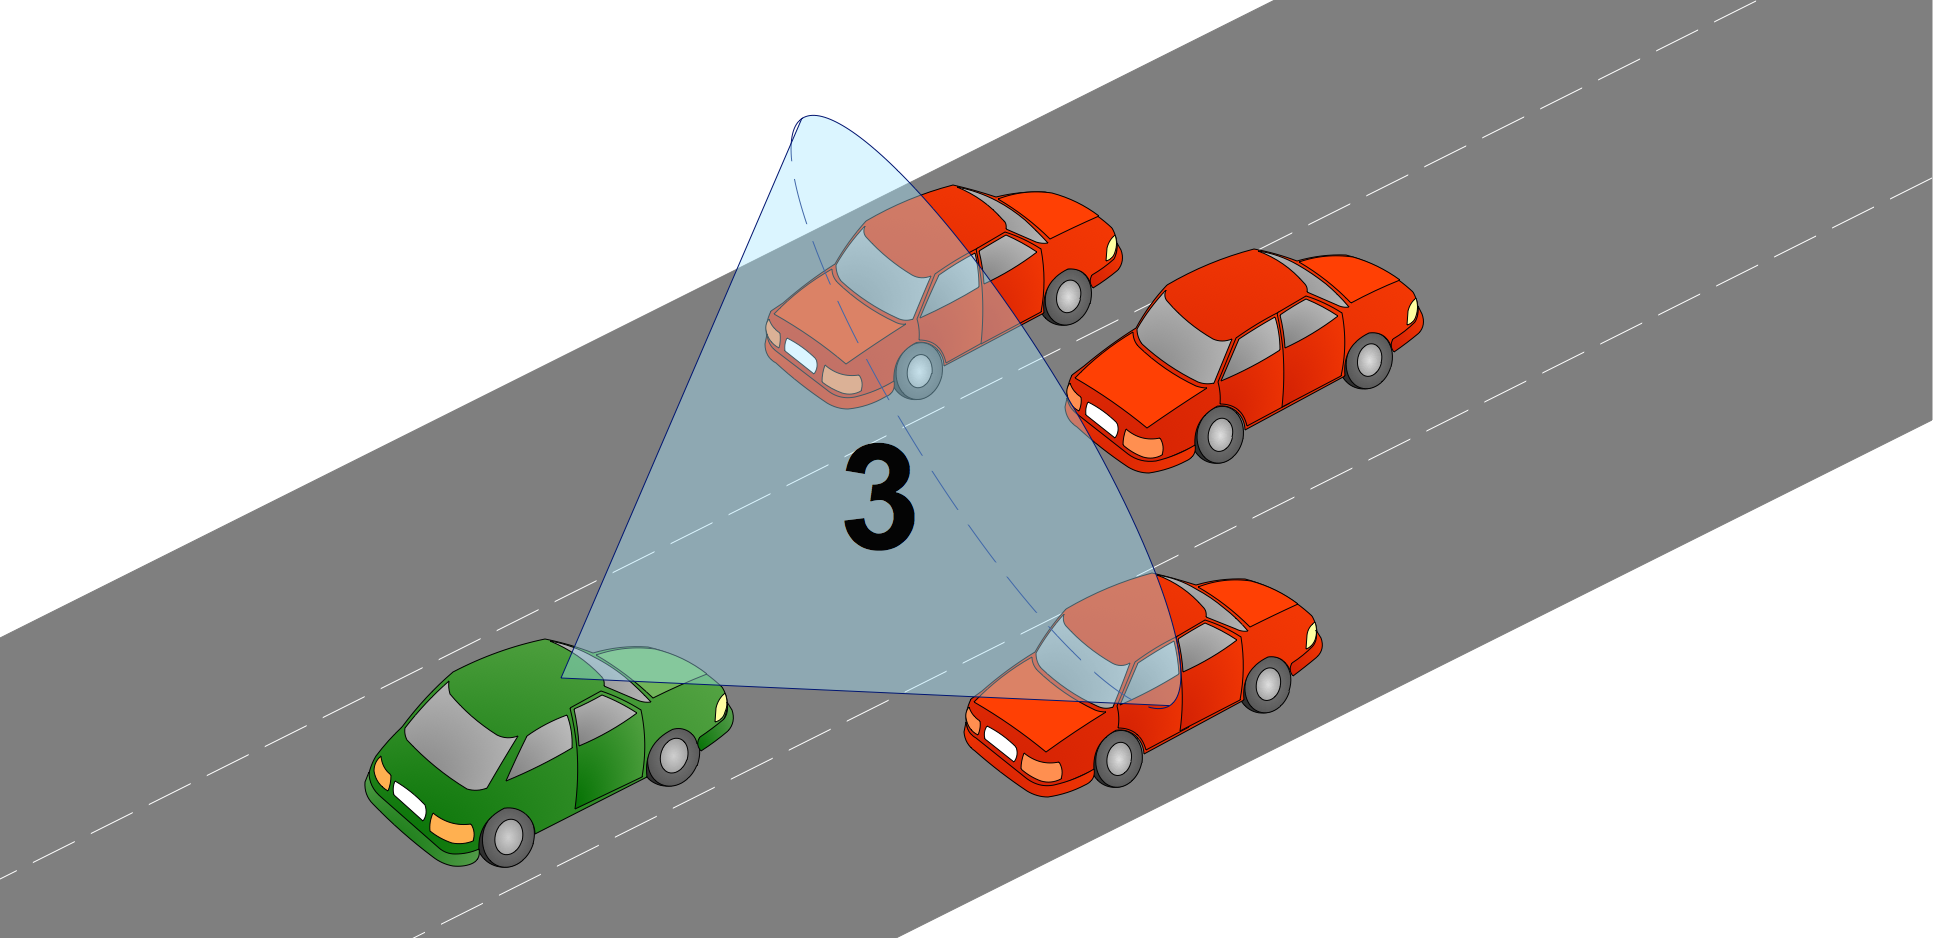
\includegraphics[width=0.28\textwidth]{text/figures/numOfObjects.png} \label{fig:introduction:semantics:a}} &
    \subfloat[Distance to rear-end of vehicle directly in front.]{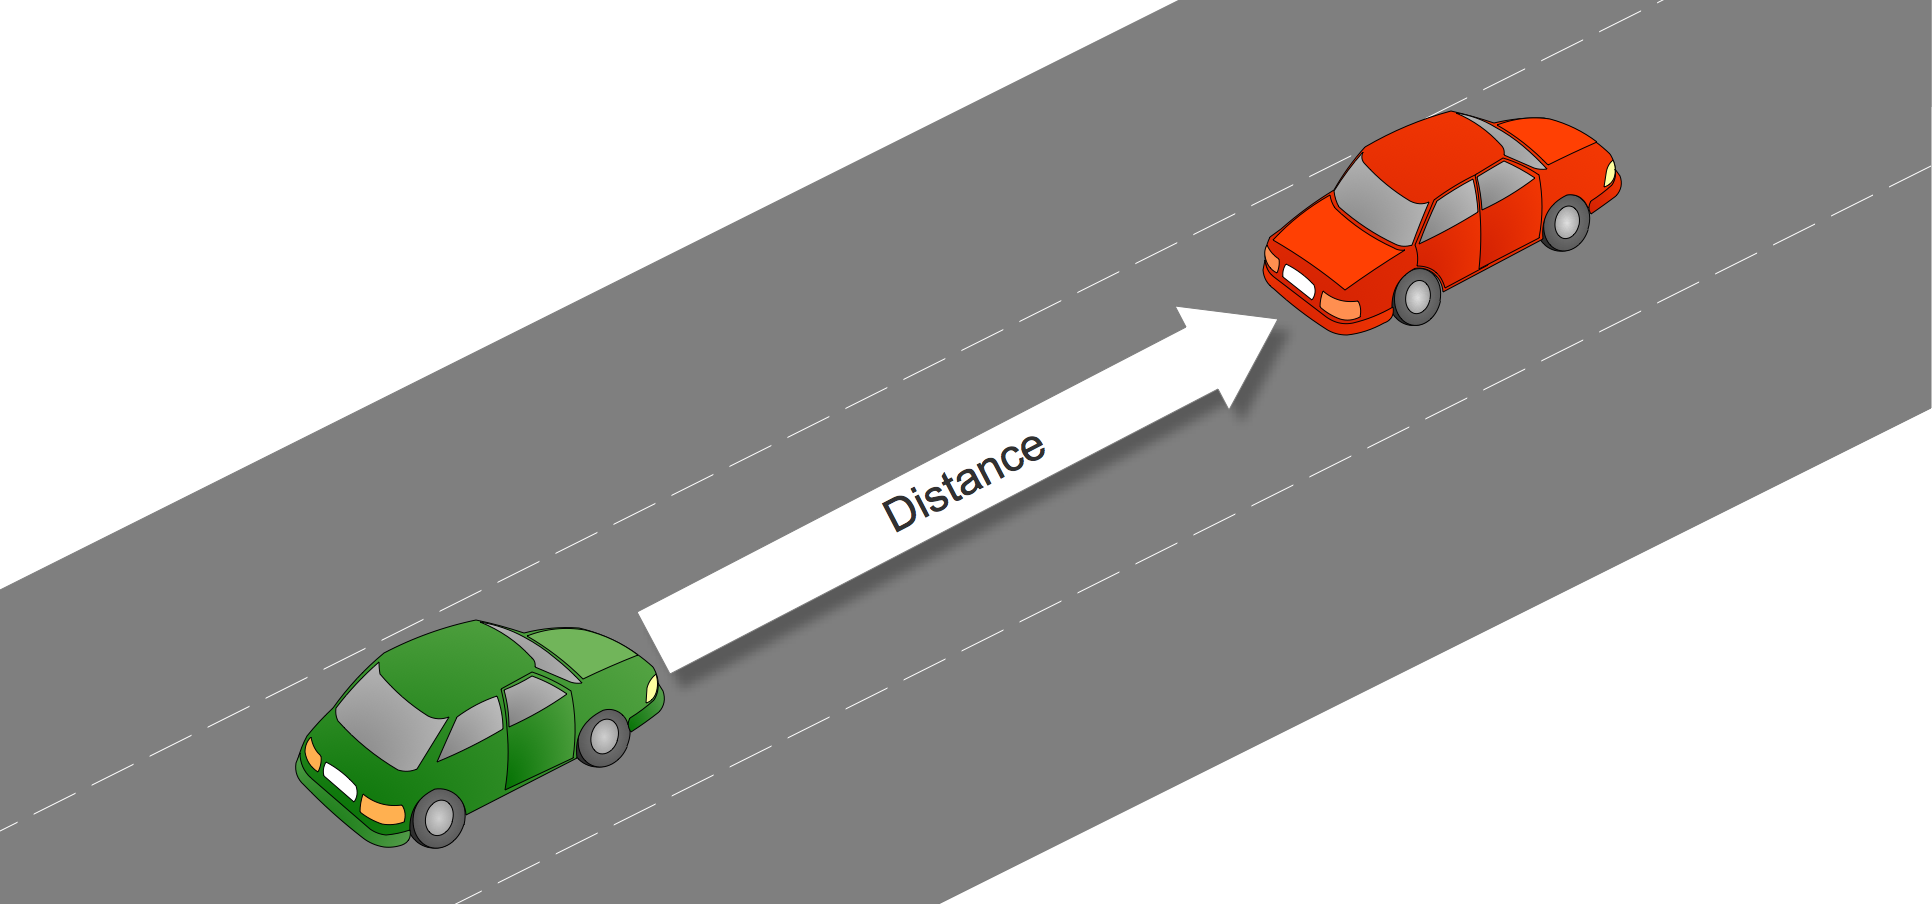
\includegraphics[width=0.28\textwidth]{text/figures/avgDistanceSameLane.png} \label{fig:introduction:semantics:b}} &
    
    \subfloat[Other vehicle entering intersection - left turn across path.]{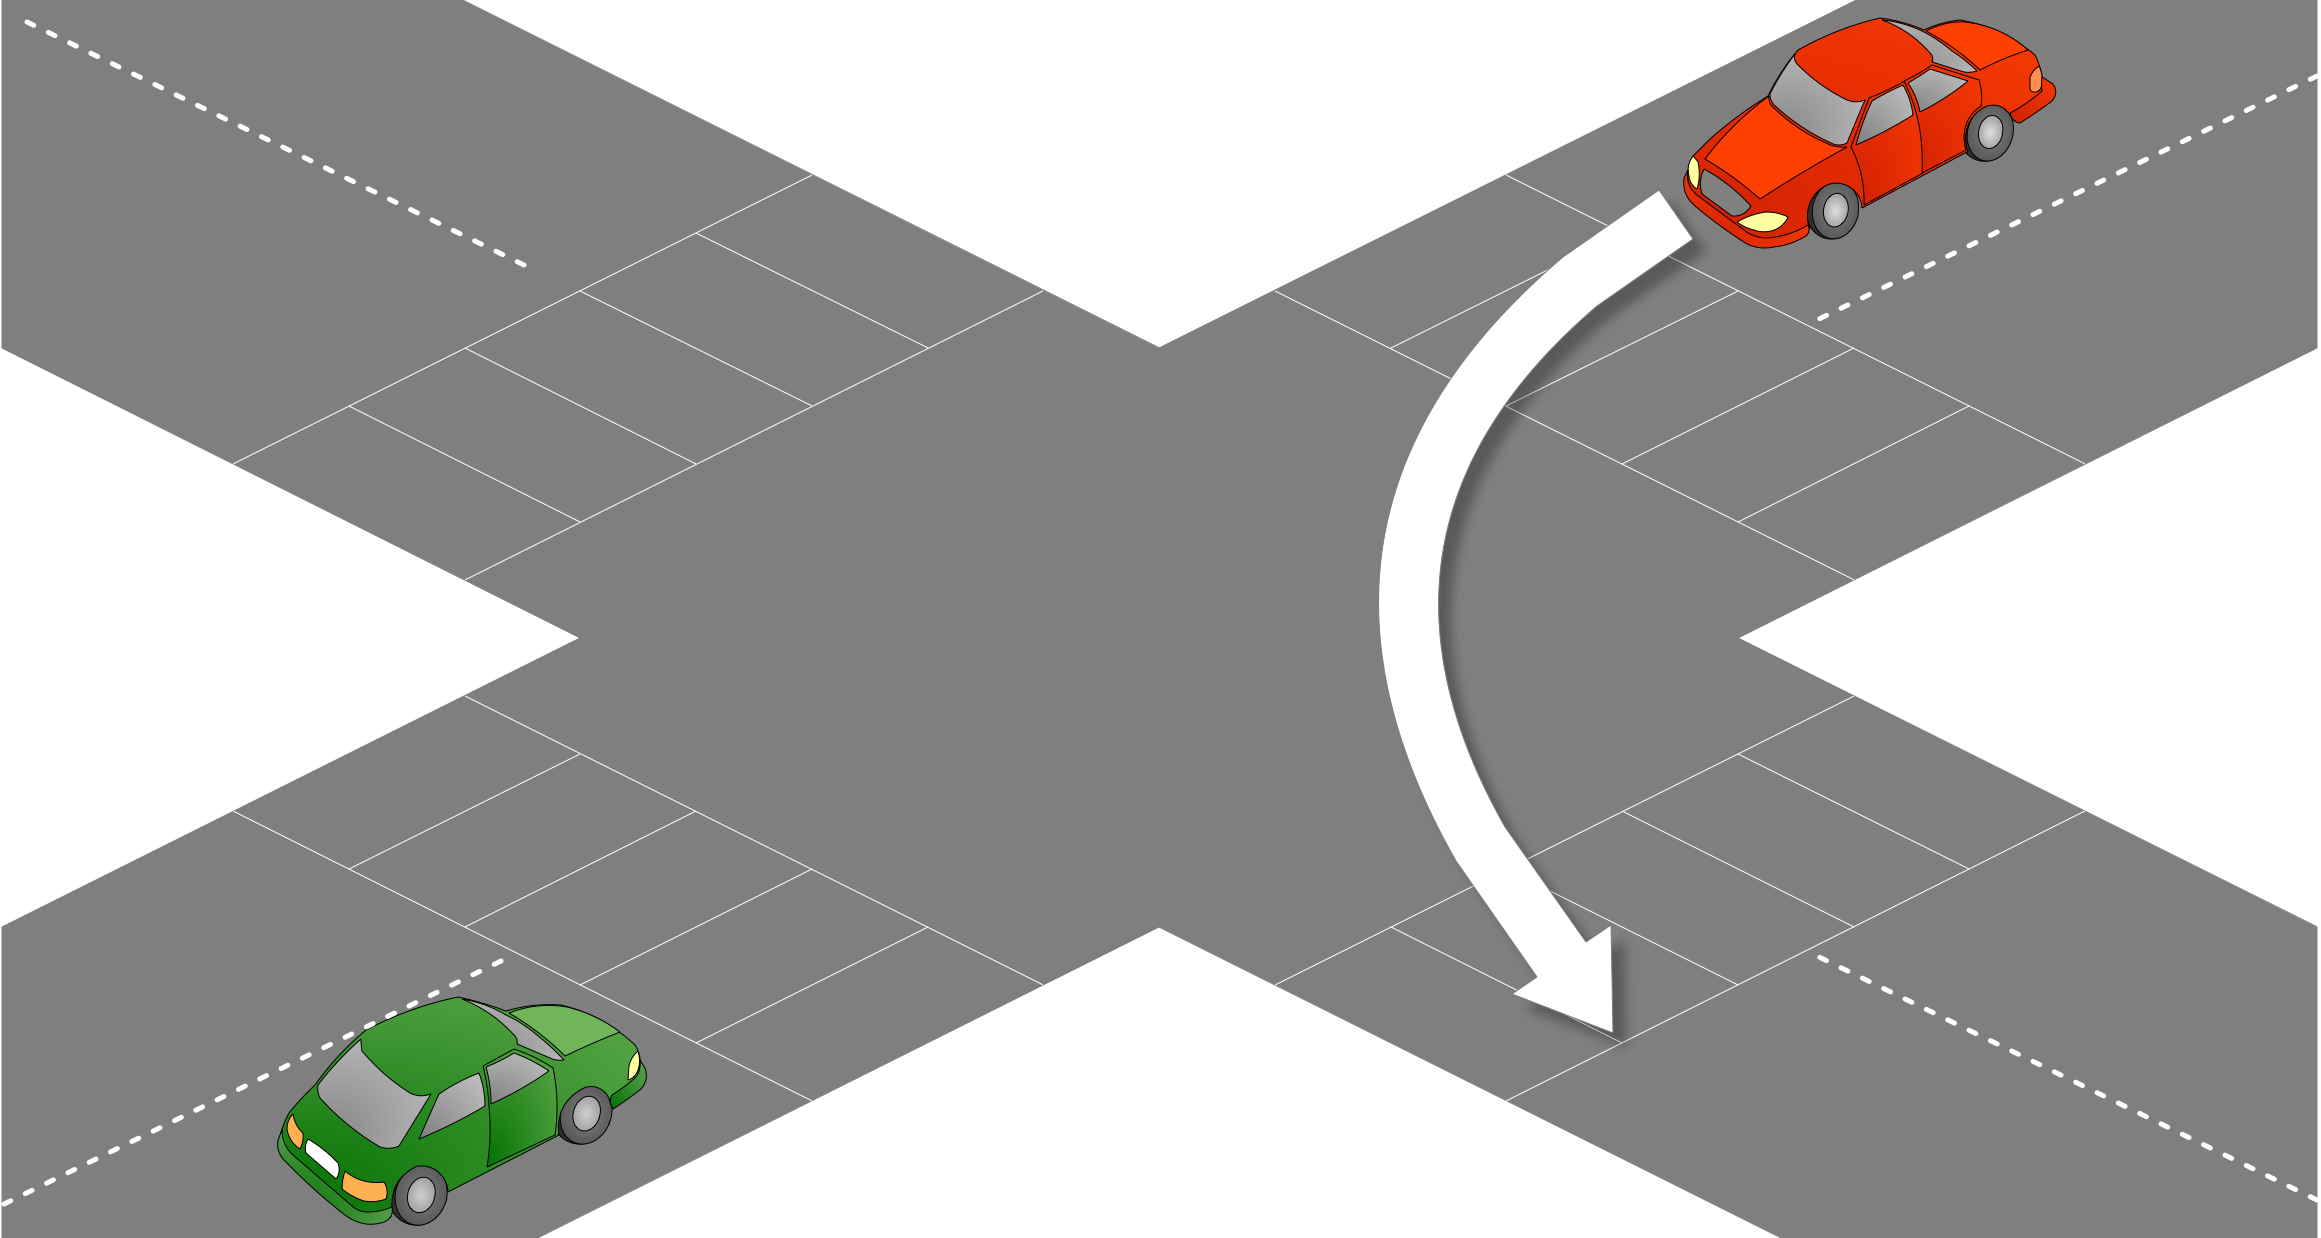
\includegraphics[width=0.28\textwidth]{text/figures/leftIntersect.png} \label{fig:introduction:semantics:c}} \\
    \subfloat[Other vehicle entering intersection - turning onto opposite direction.]{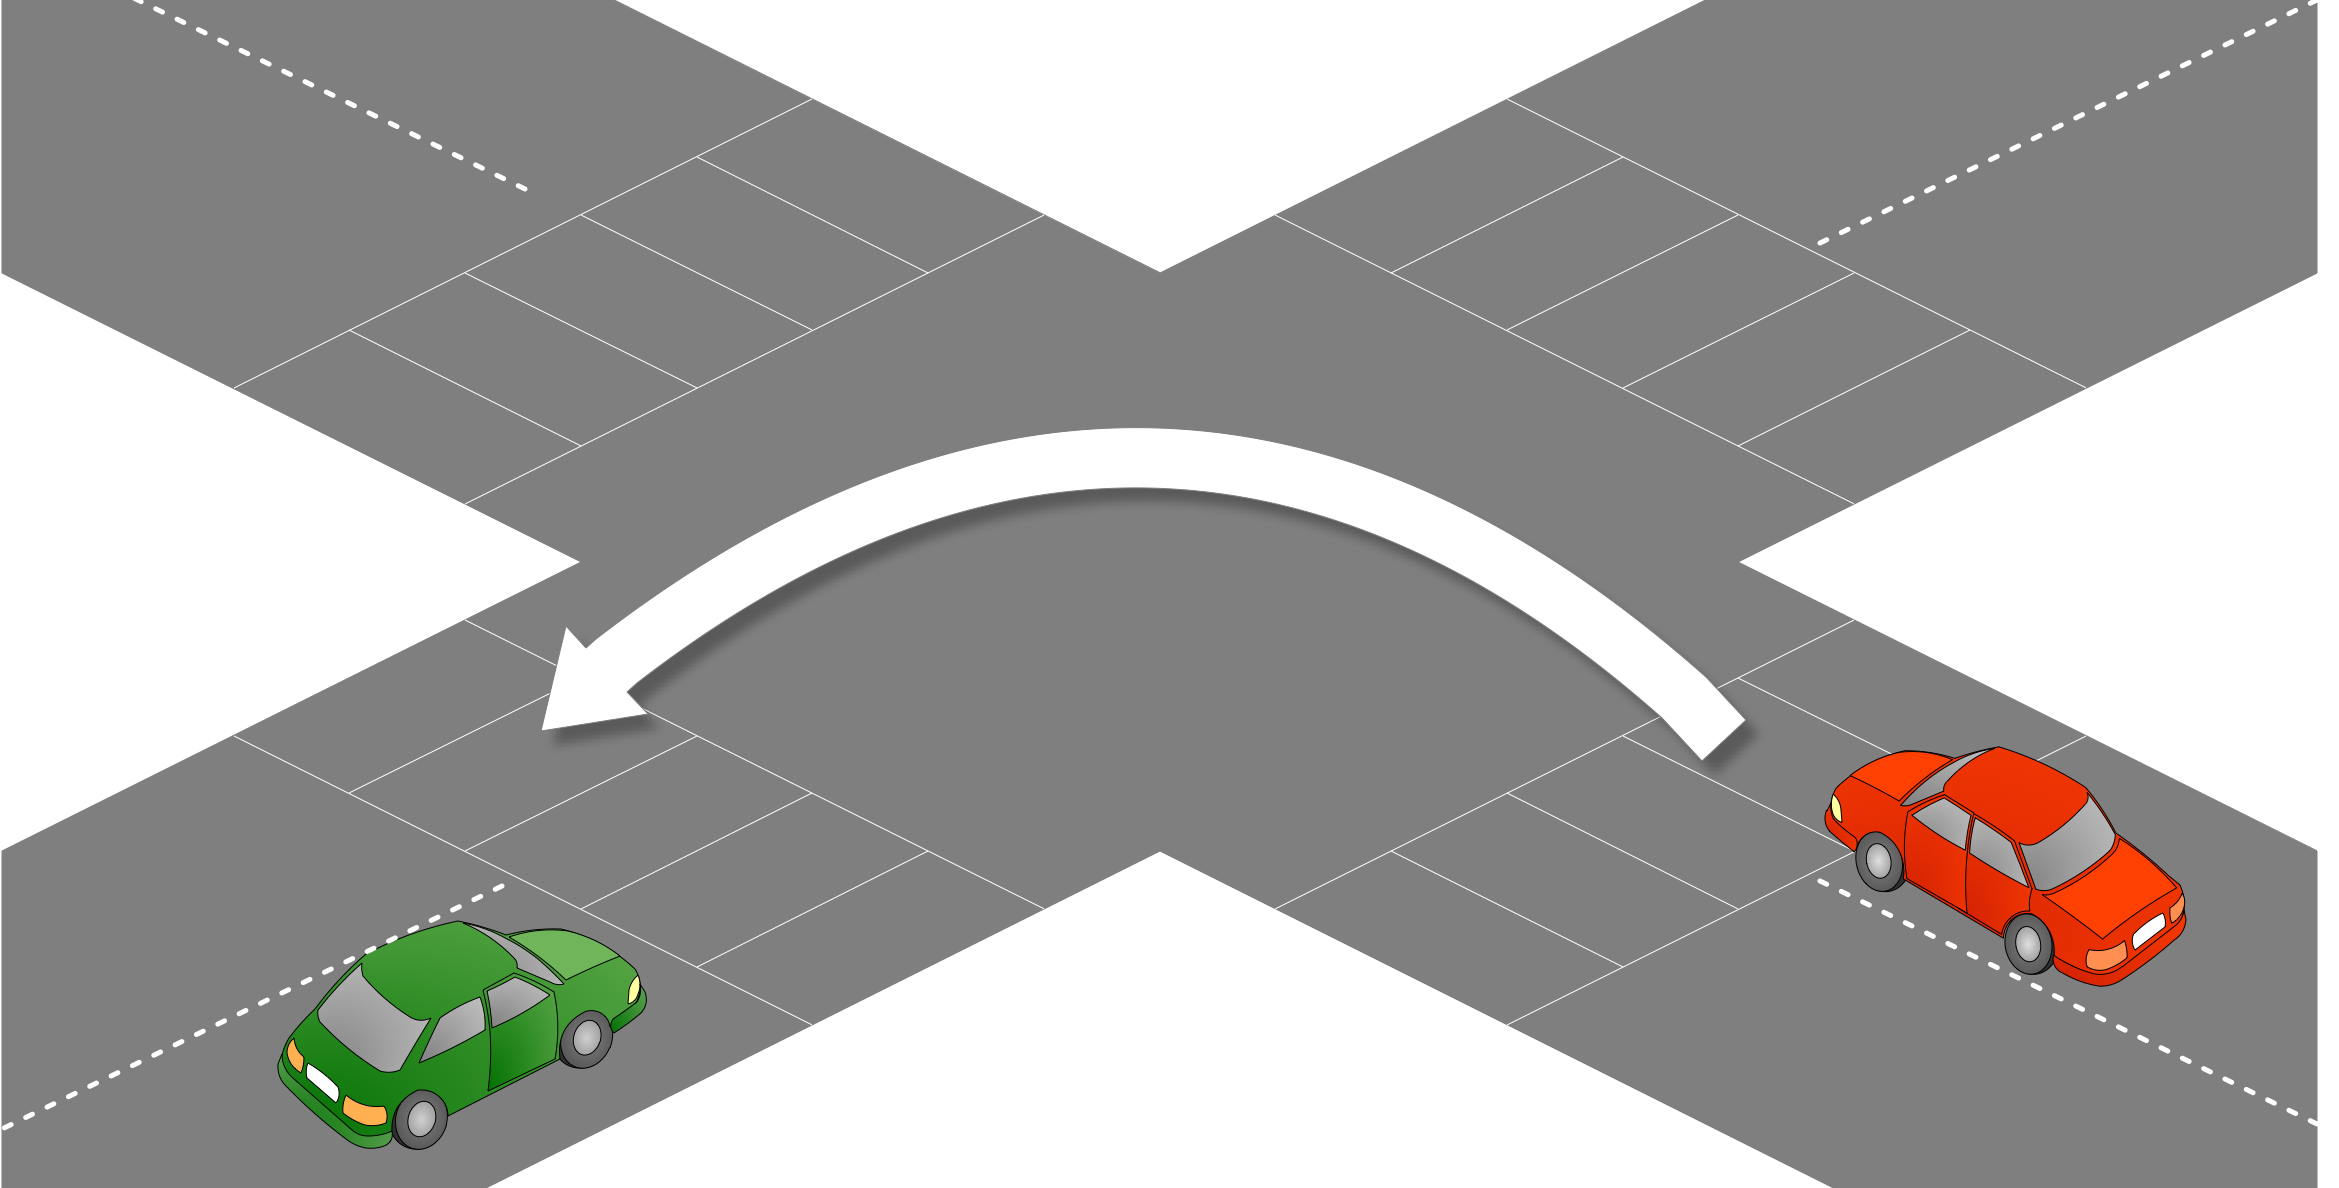
\includegraphics[width=0.28\textwidth]{text/figures/turningO.png} \label{fig:introduction:semantics:d}}&
    
    \subfloat[Other vehicle entering intersection - straight across path.]{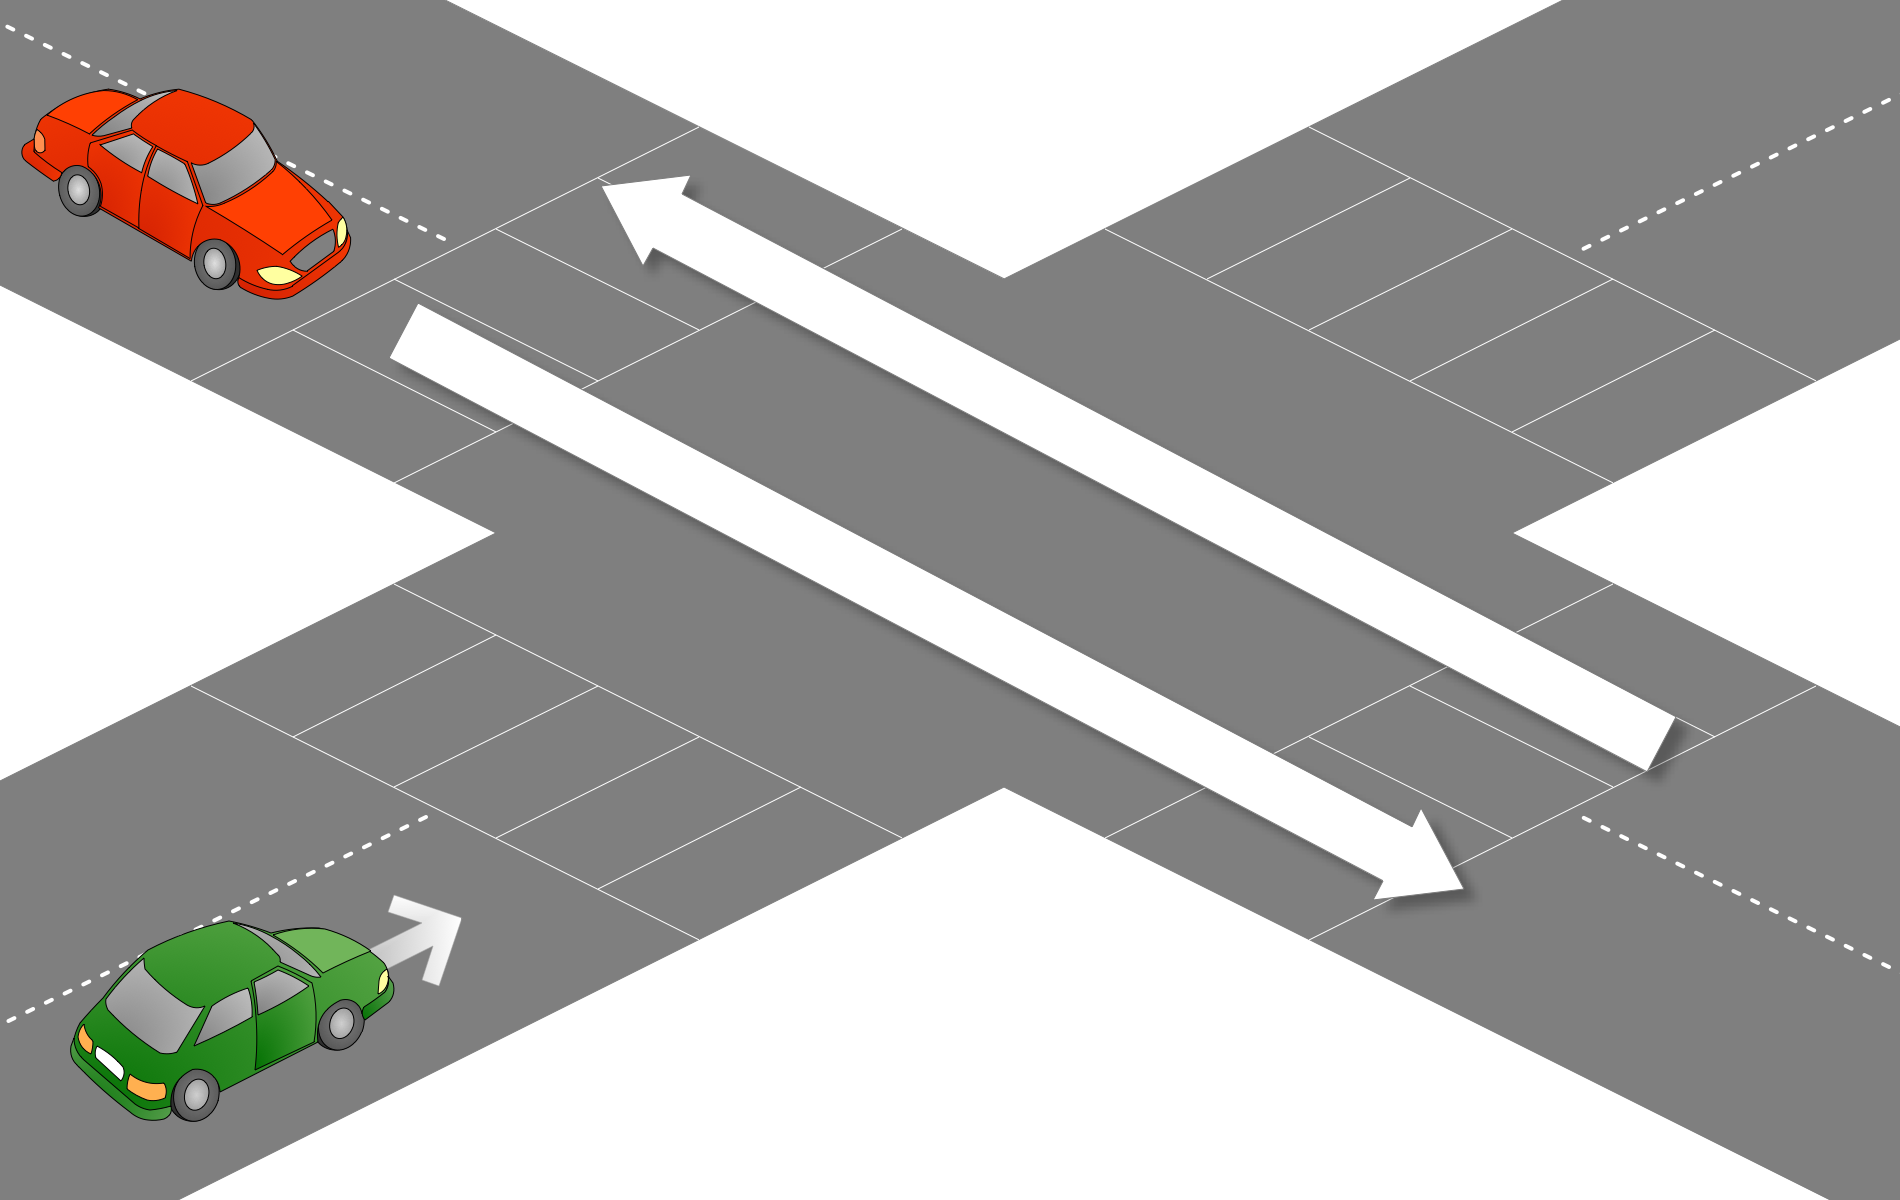
\includegraphics[width=0.28\textwidth]{text/figures/passingIntersect.png} \label{fig:introduction:semantics:e}} &
    \subfloat[Other vehicle entering intersection - turning same direction.]{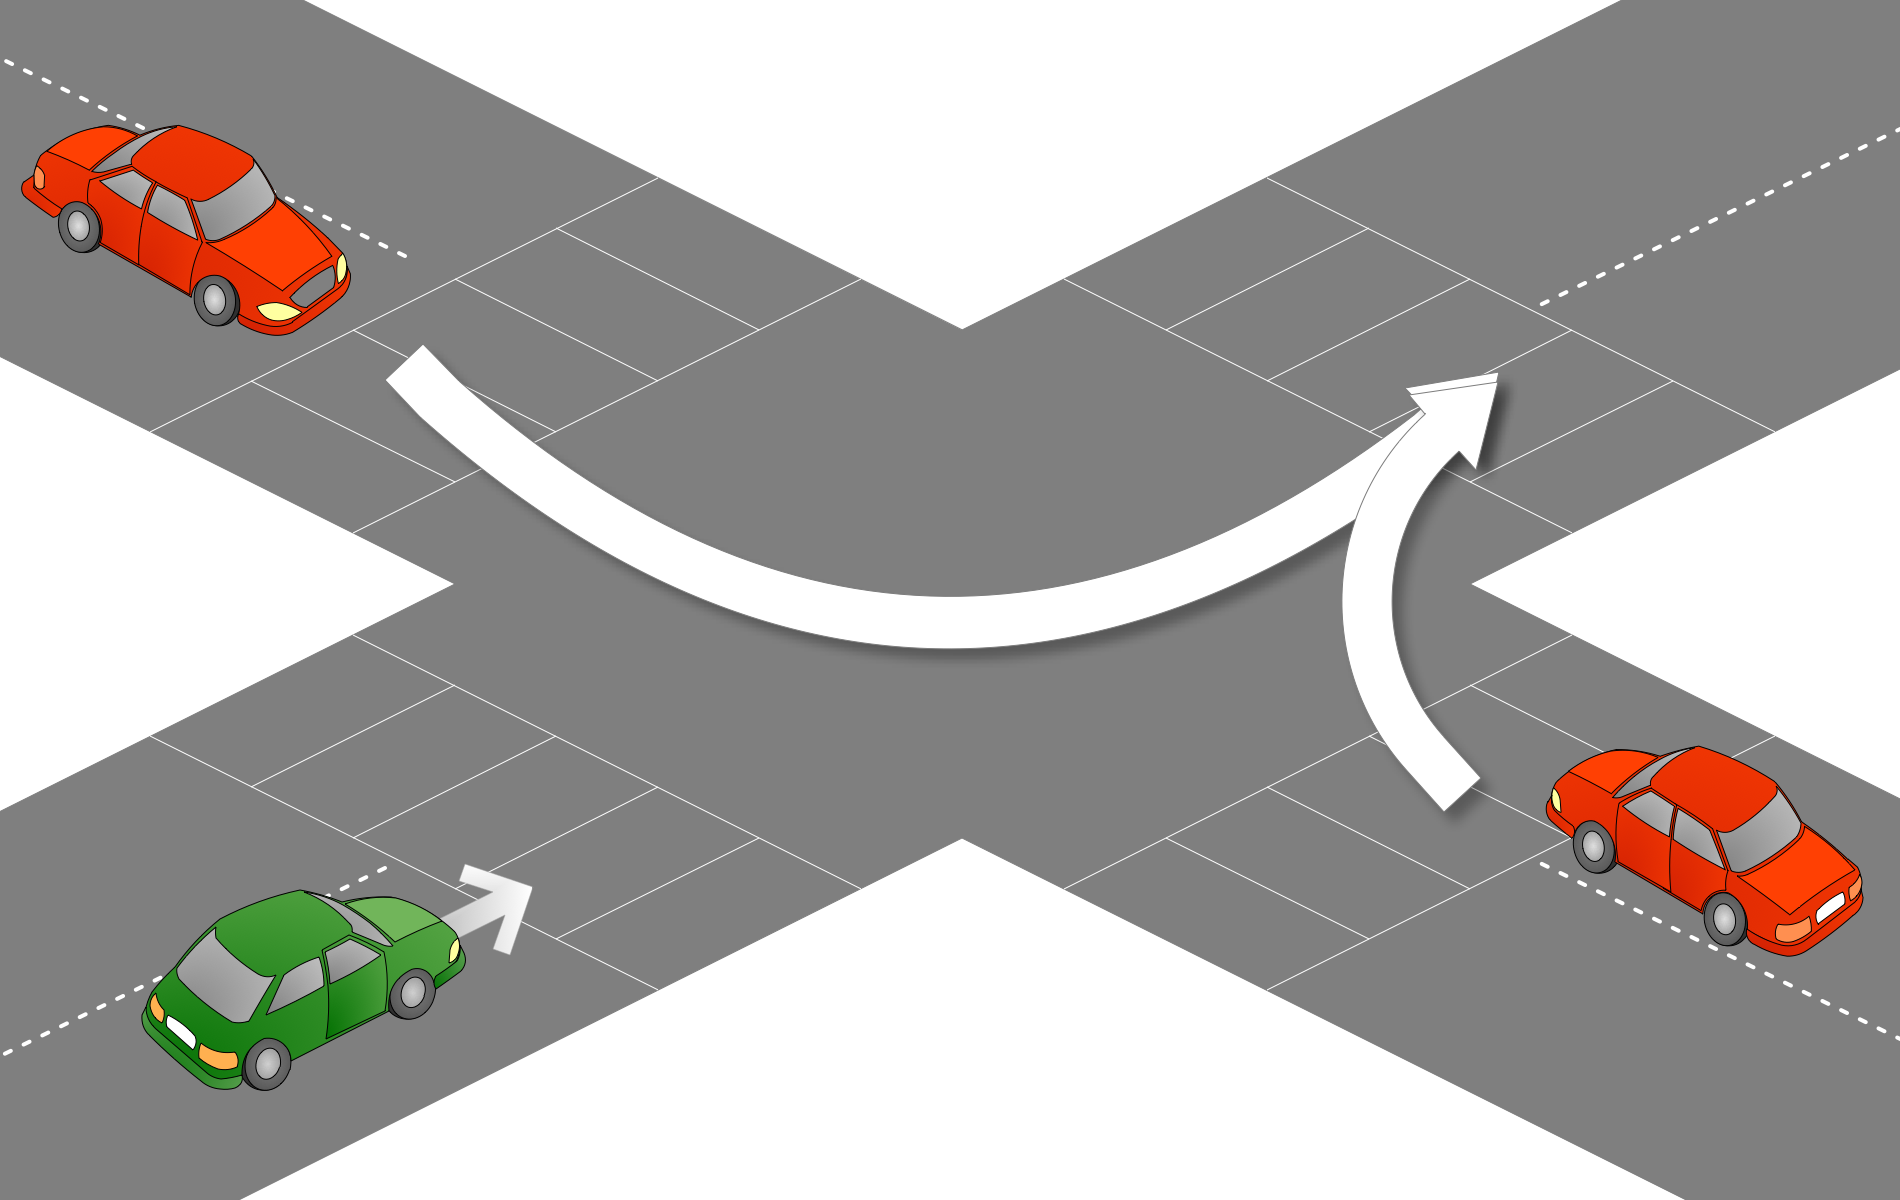
\includegraphics[width=0.28\textwidth]{text/figures/passingIntersectOntoSameDirection.png} \label{fig:introduction:semantics:f}}
  \end{tabular}
  \caption{Drive events that can be automatically detected by the method proposed in this paper. Green car is ego vehicle. Red cars are other vehicles. 
%(a) Average number of cars in front of ego-vehicle (b) Distance to rear-end of vehicle directly in front. (c) Other vehicle entering intersection - left turn across path (d) Other vehicle entering intersection - turning onto opposite direction (e) Other vehicle entering intersection - straight across path (f) Other vehicle entering intersection - turning same direction.
}
\label{fig:introduction:semantics}
\end{figure}

The contributions made with this research are:\\
\begin{itemize}
\item Using stereo-vision for automatic data reduction for NDS on both day and nighttime data, with focus on intersections (Figure \ref{fig:introduction:semantics:c}, \ref{fig:introduction:semantics:d}, \ref{fig:introduction:semantics:e}, \ref{fig:introduction:semantics:f}).
\item Introducing a new NDS event: Average number of vehicles in front of the ego vehicle. (Figure \ref{fig:introduction:semantics:a}).
\item Introducing a new NDS event: Average distance to vehicles directly in front of the ego vehicle. (Figure \ref{fig:introduction:semantics:b}).
\end{itemize}

\vspace{21.5pt}